% =====================================================================
%  SkySentry — measured values for skysentry_qcs8550_slides_v2
%
%  PART A replaces existing slides. The deck's structure is unchanged; only
%  the TBDs are filled and two factual errors corrected.
%  PART B is held back for the ablation section and is not needed to present.
%
%  Preamble additions:
%      \usepackage{booktabs}
%      \graphicspath{{docs/img/}}
%
%  Every value traces to a CSV in docs/results/; every figure to
%  4-bench/make_figures.py. Nothing here is typed in by hand.
% =====================================================================


% #####################################################################
%  PART A — replacements
% #####################################################################

% --- replaces slide 11 -------------------------------------------------
\begin{frame}{Settings and protocol}
  \begin{columns}[T,onlytextwidth]
    \begin{column}{0.5\textwidth}
      \begin{block}{Training / validation}
        \small
        \begin{tabular}{@{}ll@{}}
          Dataset   & VisDrone-DET, 208 clips \\
                    & tiled 2$\times$2, 20\% overlap \\
          Train     & 6{,}471 img $\rightarrow$ 25{,}884 tiles \\
          Val       & 548 img $\rightarrow$ 2{,}192 tiles \\
          Models    & YOLOv8n, YOLO11n, \\
                    & YOLO26n, YOLO26n-P2 \\
          Batch     & 32 \, (identical, all four) \\
          Epochs    & 30 \, (45 for P2) \\
          Seed      & 0 \\
          Image     & 640, letterbox pad 114 \\
          GPU       & A100 40\,GB \\
        \end{tabular}
      \end{block}
    \end{column}
    \begin{column}{0.46\textwidth}
      \begin{block}{Edge evaluation}
        \small
        \begin{tabular}{@{}ll@{}}
          Device    & QCS8550 \\
          Runtime   & QNN / QAIRT, W8A16 \\
          Batch     & 1 \\
          Protocol  & conf 0.001, IoU 0.65 \\
          maxDets   & 500 \, (VisDrone, not 100) \\
          Ignore    & cut per tile, masked \\
        \end{tabular}
      \end{block}
      \begin{alertblock}{Why P2 gets 45 epochs}
        \small
        \texttt{yolo26n-p2.pt} does not exist. Built from YAML with partial
        transfer from \texttt{yolo26n.pt}: \textbf{360/902} tensors, so 60\%
        starts random. Equal epochs would not be equal footing.
      \end{alertblock}
    \end{column}
  \end{columns}
\end{frame}

% --- replaces slide 12 -------------------------------------------------
\begin{frame}{Quantitative comparison}
  \begin{center}
    \small
    \begin{tabular}{@{}lrrrrrl@{}}
      \toprule
      \textbf{Model} & \textbf{Params} & \textbf{mAP} & \textbf{AP50} &
      \textbf{APs} & \textbf{QCS8550} & \textbf{Status} \\
      \midrule
      \textbf{YOLO26n-P2} & 2.662\,M & \textbf{0.2874} & \textbf{0.4766} &
        \textbf{0.1884} & 8.53\,ms & \textbf{selected} \\
      YOLO26n  & 2.572\,M & 0.2752 & 0.4631 & 0.1689 & 4.93\,ms & comparison \\
      YOLO11n  & 2.624\,M & 0.2616 & 0.4381 & 0.1556 & 4.71\,ms & comparison \\
      YOLOv8n  & 3.157\,M & 0.2606 & 0.4405 & 0.1527 & \textbf{3.98\,ms} & baseline \\
      \bottomrule
    \end{tabular}
  \end{center}
  \vfill
  \begin{columns}[T,onlytextwidth]
    \begin{column}{0.5\textwidth}
      \begin{exampleblock}{YOLO26n-P2 leads every accuracy column}
        \small
        And leads by most on \textbf{APs}: $+23.4$\% over the baseline against
        $+10.3$\% on mAP. Aerial frames are mostly small objects, so that is
        the column that matters here.
      \end{exampleblock}
    \end{column}
    \begin{column}{0.46\textwidth}
      \begin{alertblock}{YOLOv8n and YOLO11n are a tie}
        \small
        0.001 apart, and the order \emph{reverses} between runs. Not a
        difference --- reported as a tie rather than a ranking.
      \end{alertblock}
    \end{column}
  \end{columns}
  \vspace{2pt}
  \tiny\color{gray}
  mAP measured locally on 2{,}192 tiles; latency on QCS8550 via AI Hub.
  Host ms/tile omitted --- it moved 25\% between runs of the same model.
\end{frame}

% --- replaces slide 13 -------------------------------------------------
\begin{frame}{Stream inference performance on edge}
  \begin{center}
    \small
    \begin{tabular}{@{}lrrl@{}}
      \toprule
      \textbf{Stage} & \textbf{ms/tile} & \textbf{$\times$4 tiles} & \textbf{measured on} \\
      \midrule
      Letterbox resize          & 1.36 &  5.5 & board (Kryo) \\
      BGR$\rightarrow$RGB + CHW & 0.40 &  1.6 & board (Kryo) \\
      uint8 $\rightarrow$ float32 & 0.43 & 1.7 & board (Kryo) \\
      Graph execute (W8A16)     & 3.98 & 15.9 & QCS8550 (Hexagon) \\
      \textbf{Decode + NMS}     & \textbf{7.34} & \textbf{29.4} & board (Kryo) \\
      \midrule
      \textbf{Total}            & \textbf{13.52} & \textbf{54.1} &
        $\rightarrow \sim$\textbf{18\,FPS} \\
      \bottomrule
    \end{tabular}
  \end{center}
  \vfill
  \begin{center}
    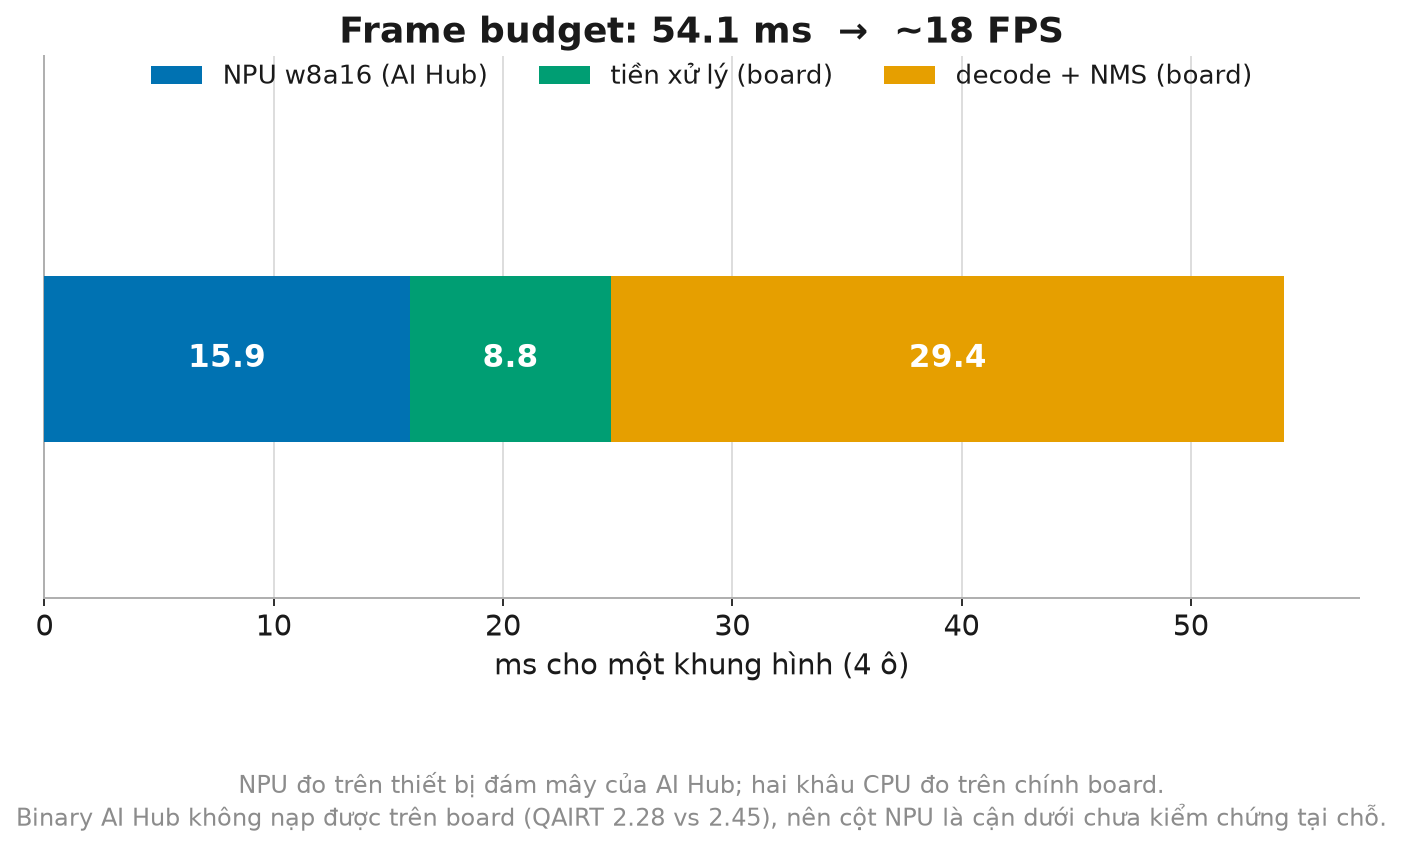
\includegraphics[width=0.86\linewidth]{fig_budget}
  \end{center}
  \vspace{-4pt}
  \begin{alertblock}{}
    \centering\small
    The NPU is \textbf{29\%} of the frame. Decode + NMS on the CPU is
    \textbf{54\%} --- larger than the entire quantized forward pass.
    Memory: \textbf{103\,MB} NPU context, \textbf{125\,MB} process RSS.
    Only detection state leaves the device, never video.
  \end{alertblock}
\end{frame}

% --- replaces slide 15 -------------------------------------------------
\begin{frame}{Ablation: does the P2 head pay for itself?}
  \begin{center}
    \small
    \begin{tabular}{@{}llrrl@{}}
      \toprule
      \textbf{Variant} & \textbf{Small objects} & \textbf{APs} &
      \textbf{Latency} & \textbf{Decision} \\
      \midrule
      YOLOv8n     & baseline             & 0.1527 & 3.98\,ms & reference \\
      YOLO11n     & newer backbone       & 0.1556 & 4.71\,ms & tie with baseline \\
      YOLO26n     & NMS-free head        & 0.1689 & 4.93\,ms & $+10.6$\% APs \\
      \textbf{YOLO26n-P2} & \textbf{+ stride-4 branch} & \textbf{0.1884} &
        8.53\,ms & \textbf{$+23.4$\% APs} \\
      \bottomrule
    \end{tabular}
  \end{center}
  \vfill
  \begin{columns}[T,onlytextwidth]
    \begin{column}{0.5\textwidth}
      \begin{block}{What the stride-4 branch costs}
        \small
        Anchors go from \textbf{8{,}400 to 34{,}000} at 640\,px. Latency
        $3.98 \rightarrow 8.53$\,ms (2.1$\times$) for only 3.5\% more weights.
        The cost is resolution, not parameters.
      \end{block}
    \end{column}
    \begin{column}{0.46\textwidth}
      \begin{exampleblock}{Answer}
        \small
        Over the whole pipeline the extra 4.55\,ms/tile costs
        \textbf{18.5 $\rightarrow$ 13.8\,FPS}, a \textbf{25\% throughput loss}.
        Worth it if the requirement is $\sim$12\,FPS; not if it is 15 or more.
        \textbf{The frame-rate requirement decides, not the mAP table.}
      \end{exampleblock}
    \end{column}
  \end{columns}
\end{frame}


% #####################################################################
%  PART B — two corrections to existing slides (edit in place, no new frame)
% #####################################################################
%
%  SLIDE 9 — remove two rungs from the evaluation ladder.
%    "W8A8 + INT16 head" and "lite_mp 10% INT16" are per-layer mixed
%    precision. AI Hub's submit_quantize_job takes one dtype pair for the
%    whole model, and Qualcomm documents mixed precision as "currently not
%    supported". Replace the five-rung ladder with:
%
%        0  FP32 CPU reference
%        1  W8A8
%        2  W8A16      <- the only precision usable on every model
%        3  W16A16
%        4  W4A16
%
%  SLIDE 16 — "Quantization may damage detection heads" is now measured, so
%    change "may damage" to "does damage" and add the figure:
%        W8A8 collapses the classification head on 5 of 5 model/export
%        combinations -- every class score exactly 0.0 while box regression
%        stays healthy. 8 of 16 quantized configurations are unusable and
%        every one of them reports good latency with zero operator fallback.
%
%  SLIDE 4 — tracking and counting are training-free (ByteTrack + Kalman);
%    only detection is trained. Worth stating: it is a deployment choice, not
%    a gap, and it costs no extra inference pass on the edge device.
%
% #####################################################################
%  PART C — held back for the ablation section. Not needed to present.
%     docs/img/fig_quant_trap.png   the fastest precision is the broken one
%     docs/img/fig_e2e_matrix.png   YOLO26 cannot be quantized end-to-end
%     docs/img/fig_power.png        three power counters, none usable
%     docs/img/fig_pipeline.png     pipeline with per-stage timings
%     docs/img/fig_tradeoff.png     accuracy vs NPU latency
%  Full write-up: docs/EDGE_BENCHMARK.md
% #####################################################################
